\section{Discussion and Conclusion}\label{sec:conclusion}

We have measured the local PNG parameter $\fnl$ using the scale-dependent bias in the angular clustering of LRGs selected from the DESI Legacy Imaging Survey DR9. Our sample includes more than $12$ million LRG targets covering around $14,000$ square degrees in the redshift range of $0.2< z < 1.35$. We leverage early spectroscopy during DESI Survey Validation \citep{desi2023sv} to infer the redshift distribution of our sample (Figure \ref{fig:nz}). In our fiducial analysis, we have obtained a maximum likelihood value of $\fnl=47$ with a significant probability that $\fnl$ is greater than zero, $P(\fnl>0)=99.9$ (Figure \ref{fig:mcmc_dr9} and Table \ref{tab:dr9methodcalib}). 

The signature of local PNG is very sensitive to excess clustering signals caused by imaging systematic effects. \mout{We have applied a series of robustness tests on the impact of how we estimate the selection function of our LRG sample, including: the methods (linear and nonlinear), the set of imaging systematic maps used (Galactic extinction, stellar density, depth in $grzW1$, psfsize in $grz$, and neutral hydrogen column density), and data quality cuts on the accepted regions}. \mr{We have applied a series of robustness tests to investigate the impact of how the galaxy selection function is determined. Specifically, both linear and nonlinear methods are applied using various combinations of imaging systematic maps (Galactic extinction, stellar density, depth in $grzW1$, psfsize in $grz$, and neutral hydrogen column density). We also examine the effect of different masks based on imaging.} \mr{Overall, we} find no change in the analysis that shifts the maximum likelihood value of $\fnl$ to a significantly lower value (Figure \ref{fig:mcmc_dr9reg}, Figure \ref{fig:mcmc_dr9elmin}, and Table \ref{tab:dr9method}). The only manner in which the significance of nonzero PNG decreases is due to the uncertainty on the measurement increasing when we employ more imaging systematic maps \mr{for} the selection function estimation and by doing so remove large-scale clustering information (the effect of which on $\fnl$ recovery we have calibrated with mocks, as shown in Figure \ref{fig:fnlbias}).

\begin{figure}
    \centering
    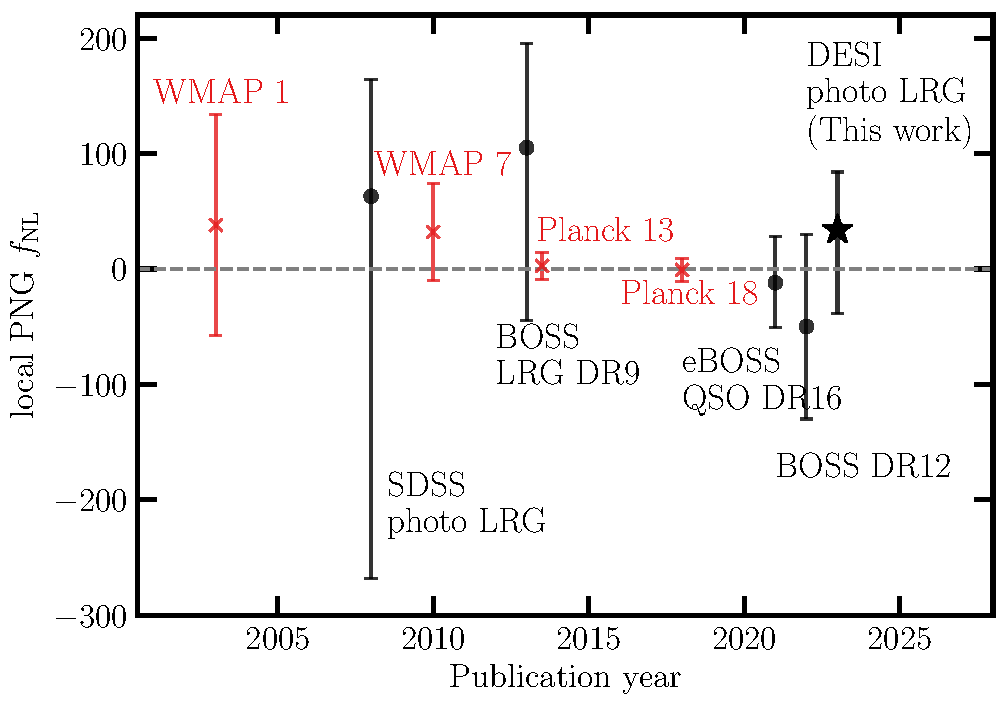
\includegraphics[width=0.45\textwidth]{figures/fnl_history.pdf}
    \caption{History of constraints on local PNG $\fnl$ at $95\%$ confidence from single-tracer LSS \citep{slosar2008constraints,2013MNRAS.428.1116R, mueller2022primordial}, including our analysis with $25<\fnl<76$ (DESI photo LRG) and CMB surveys \citep{Komatsu_2003, Komatsu_2010, planck13, akrami2019planck}. The median $\fnl$ value is used in case the maximum likelihood estimate was not reported in the reference.}
    \label{fig:fnlhist}
\end{figure}

When comparing our fiducial results to recent CMB and QSO measurements, as shown in Figure \ref{fig:fnlhist}, we find a \mr{significant} tension with CMB but consistent constraints with LSS within $95\%$ confidence. Either we have measured an $\fnl$ signal that is inconsistent with CMB measurements or there is a hidden source of systematic contamination in our data which cannot be mitigated with available imaging systematic maps. \mr{To be consistent with CMB measurements, our results would need to correspond to some kind of scale-dependent $\fnl$ model which has a larger non-gaussianity on LSS scales but negligible one at CMB scales \citep{sefusatti_2009, becker_2011}}. Our analysis can be considered as the first attempt to identify major systematics in DESI, so we can be ready for constraining $\fnl$ with DESI spectroscopy. Internal DESI tests of the photometric calibration \mout{are}\mr{were} unable to uncover DESI-specific issues, e.g., when comparing to Gaia data. The most significant trends that we find are with the E(B-V) map. The source of such a trend would be a mis-calibration of the E(B-V) map itself or the coefficients applied to obtain Galactic extinction corrected photometry. \mout{Such issues are generically likely to be proportional in amplitude to the estimated E(B-V), but may not strictly follow the estimated E(B-V)}\mr{Such a mis-calibration would plausibly be proportional in amplitude to the estimated E(B-V) map, though it may not have E(B-V)’s spatial distribution.} In order to explain the $\fnl$ signal we measure, such an effect would need to be approximately twice that of the trend we find with E(B-V). There are ongoing efforts within DESI to obtain improved Galactic extinction information, which will help \mout{discover}\mr{establish} if this is indeed the cause.


%Discuss generic effect of calibration. Ask Rongpu if we can include the Gaia calibration test map, which shows patterns that look related to the Gaia scanning strategy, rather that Legacy Survey? (If not, we can just say something like "internal DESI tests of the photometric calibration are unable to uncover DESI-specific issues, e.g., when comparing to Gaia data") Then, something like "The most significant trends that we find are with the E(B-V) map. The source of such a trend would be a mis-calibration of the E(B-V) map itself or the coefficients applied to obtain Galactic extinction corrected photometry. Such issues are generically likely to be proportional in amplitude to the estimated E(B-V), but may not strictly follow the estimated E(B-V). In order to explain the fNL signal we measure, such an effect would need to be approximately twice that of the trend we find with E(B-V). There are ongoing efforts within DESI to obtain improved Galactic extinction information, which will help discover if this is indeed the cause. (Anything to say about Mudur et al. map? I think we need to write something. Perhaps for now just something like "a first look at the Mudur et al E(B-V) maps did not suggest including them would change our results" and then during CWR you could add Mudur-SFD as a map to test against?)"



%We have presented constraints on the local primordial non-Gaussianity parameter $\fnl$ from the angular power spectrum of LRGs from the DESI imaging DR9.  Our LRG sample includes more than $14$ million targets covering around $18,000$ square degrees in the redshift range of $0.2< z < 1.35$. Our analysis utilizes the scale-dependent bias effect that primarily comes from large scales; thus, it is very sensitive to systematic errors caused by photometric calibration issues, survey depth variations, and Milky Way foregrounds (Figure \ref{fig:ng}). 

%We use the FFTLog algorithm to model the angular clustering on large scales or multipoles as low as $\ell=2$ (Figure \ref{fig:model_mock}). We simulate lognormal density fields with DESI-like LRG angular and redshift distributions to validate the pipeline, estimate covariance matrices, and characterize remaining systematic errors. Our mock test reveals that the distribution of power spectra on large scales is asymmetric (Figure \ref{fig:histcell}). We demonstrate our likelihood inference benefits from fitting the log transformation of the power spectrum. %Multivariate linear and neural network-based regression models are applied to regress out spurious fluctuations in the LRG density field against various maps for the extinction, survey depth, astronomical seeing, neutral hydrogen column density, and stellar density. Feature selection uses the Pearson correlation and the Spearman correlation coefficients to reduce the likelihood of over-correction, i.e., removing the clustering signal (Figure \ref{fig:pcc}). The LRG density map is cross-correlated against the imaging systematic maps (Figure \ref{fig:clxmock}), and the mean LRG density is calculated for different regions with similar imaging to look for systematic trends in the mean density (Figure \ref{fig:nbarmock}). Using the mean density and cross-power spectrum diagnostics, we quantify the remaining systematics against lognormal simulations (Figure \ref{fig:chi2test}). We identify the extinction, z-band depth, and r-band seeing as the primary sources of systematic error. Our simulation-based tests reveal that the DESI LRG targets cleaned with linear three maps suffers from significant remaining systematic error primarily due to depth variations. We observe that the non-linear mitigation approach reduces the excess clustering signal more effectively. 

%We apply our cleaning methods to the lognormal mocks with and without PNG, with and without systematic effects, to calibrate the level of mitigation biases introduced in our constraints (Table \ref{tab:debiasparams} and Figure \ref{fig:fnlbias}). With three maps, we obtain best-fitting estimates which are inconsistent with zero at more than $95\%$ confidence. Adding local stellar density to the list of maps used for cleaning the LRG sample does not influence the constraints. However, using the combination of all imaging systematic maps and stellar density yields an asymmetric likelihood distribution with larger uncertainty and consistent with $\fnl=0$ at $95\%$ confidence (Table \ref{tab:dr9methodcalib}), which is interesting as the same covariance matrix is used for all; but we find that the \textit{non-linear nine maps} approach introduces a larger bias by having a larger multiplicative parameter, $m_{1}$, Table \ref{tab:debiasparams}. Overall, our non-linear cleaning methods return consistent best-fitting estimates of $\fnl \sim 47-50$ (Figure \ref{fig:mcmc_dr9}). We run multiple robustness tests but find no significant changes other than that there is spurious correlation against stellar density in the NGC and potential calibration issues in the SGC below DEC$< -30$ (Table \ref{tab:dr9method}). Our constraints are consistent with each other when each imaging region is fit separately and/or the lowest mode used is increased (Figure \ref{fig:mcmc_dr9reg} and Figure \ref{fig:mcmc_dr9elmin}). Assuming Planck's measurement of $\fnl$ is accurate a priori, our results indicate some unknown systematic effects. \mr{Santi: Potentially, this could also indicate a more complicated type of PNG (scale dependent, beyond quadratic fnl, non-local...) I would also discuss possible implications from assuming a different cosmology.} Our results also suggest follow-up investigations of stellar contamination and depth-related variations in the spectroscopic sample of DESI LRGs. \mr{Hui: cite LRG redshift success rate, stellar contamination rate. Noting possible improvements when we have all spectra data available.} On the other hand, calibrating simulations for the over-correction effect might not be feasible for DESI spectroscopy. So, a simulation-based forward-model approach for estimating the imaging weights can become helpful to reduce the dimensionality of the imaging parameter space. We leave the idea of combining the forward-modeling and backward-modeling cleaning approaches to future work.